\section{Results}
Figure~\ref{fig:subspace-tradeoff} compares the matched recovery-radius medians before and after the feature-subspace stage-2 defense. The defense improves BalDRO, SalUn, and ORBIT, while RURK remains hard and SCRUB behaves like generic adversarial fragility.

\begin{figure}[t]
  \centering
  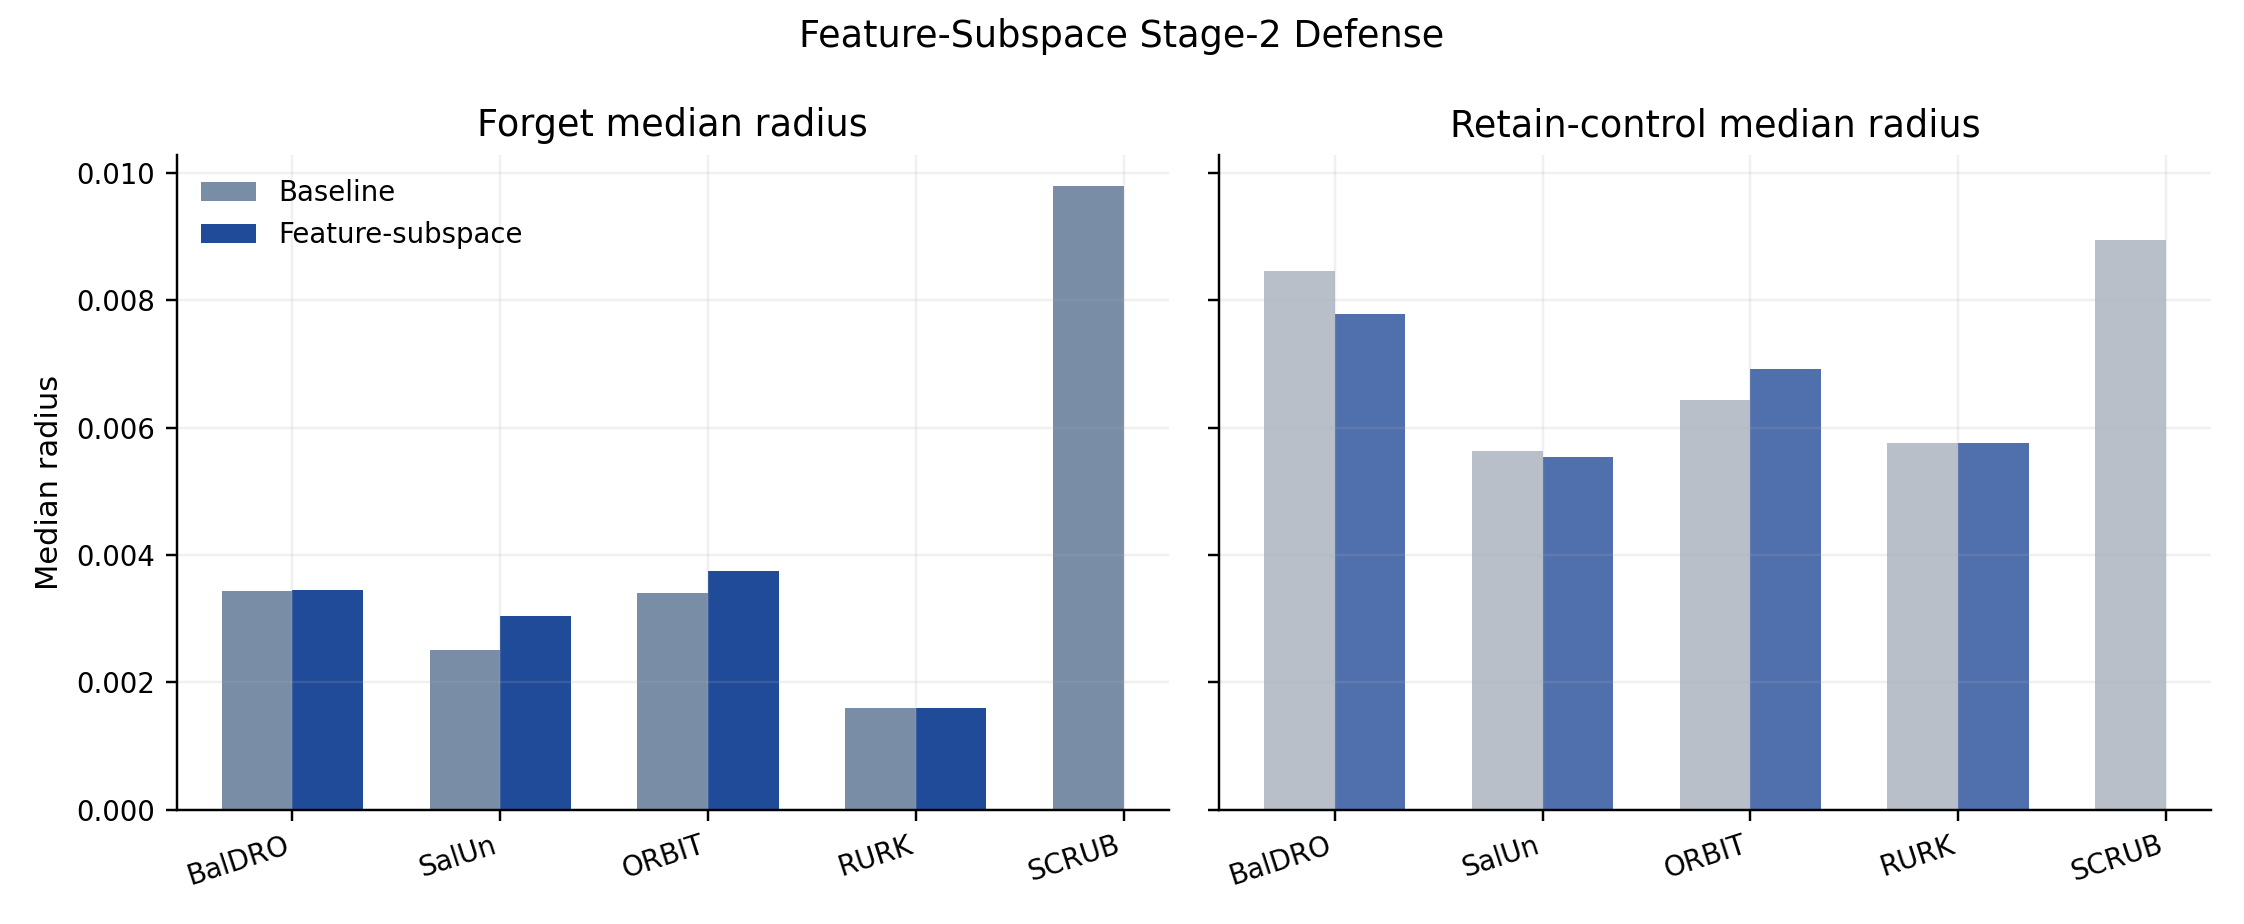
\includegraphics[width=0.9\linewidth]{feature_subspace_tradeoff.png}
  \caption{Forget/retain recovery medians under the feature-subspace stage-2 defense.}
  \label{fig:subspace-tradeoff}
\end{figure}

\begin{figure}[t]
  \centering
  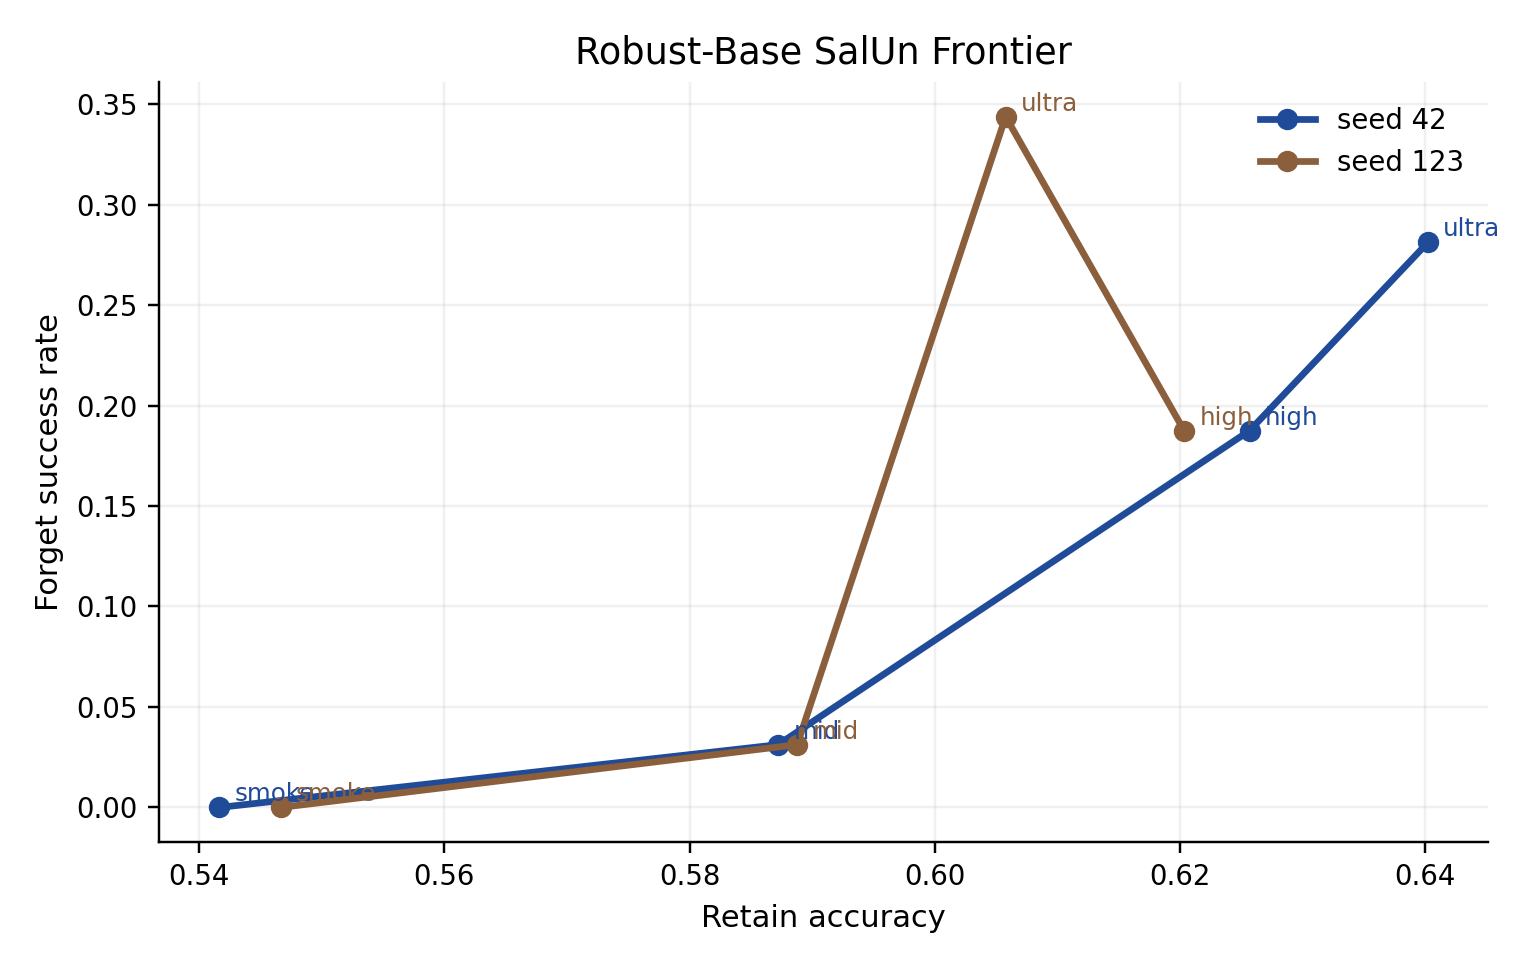
\includegraphics[width=0.9\linewidth]{robust_base_frontier.png}
  \caption{Utility-vs-recovery frontier for robust-base SalUn.}
  \label{fig:robust-frontier}
\end{figure}

\begin{figure}[t]
  \centering
  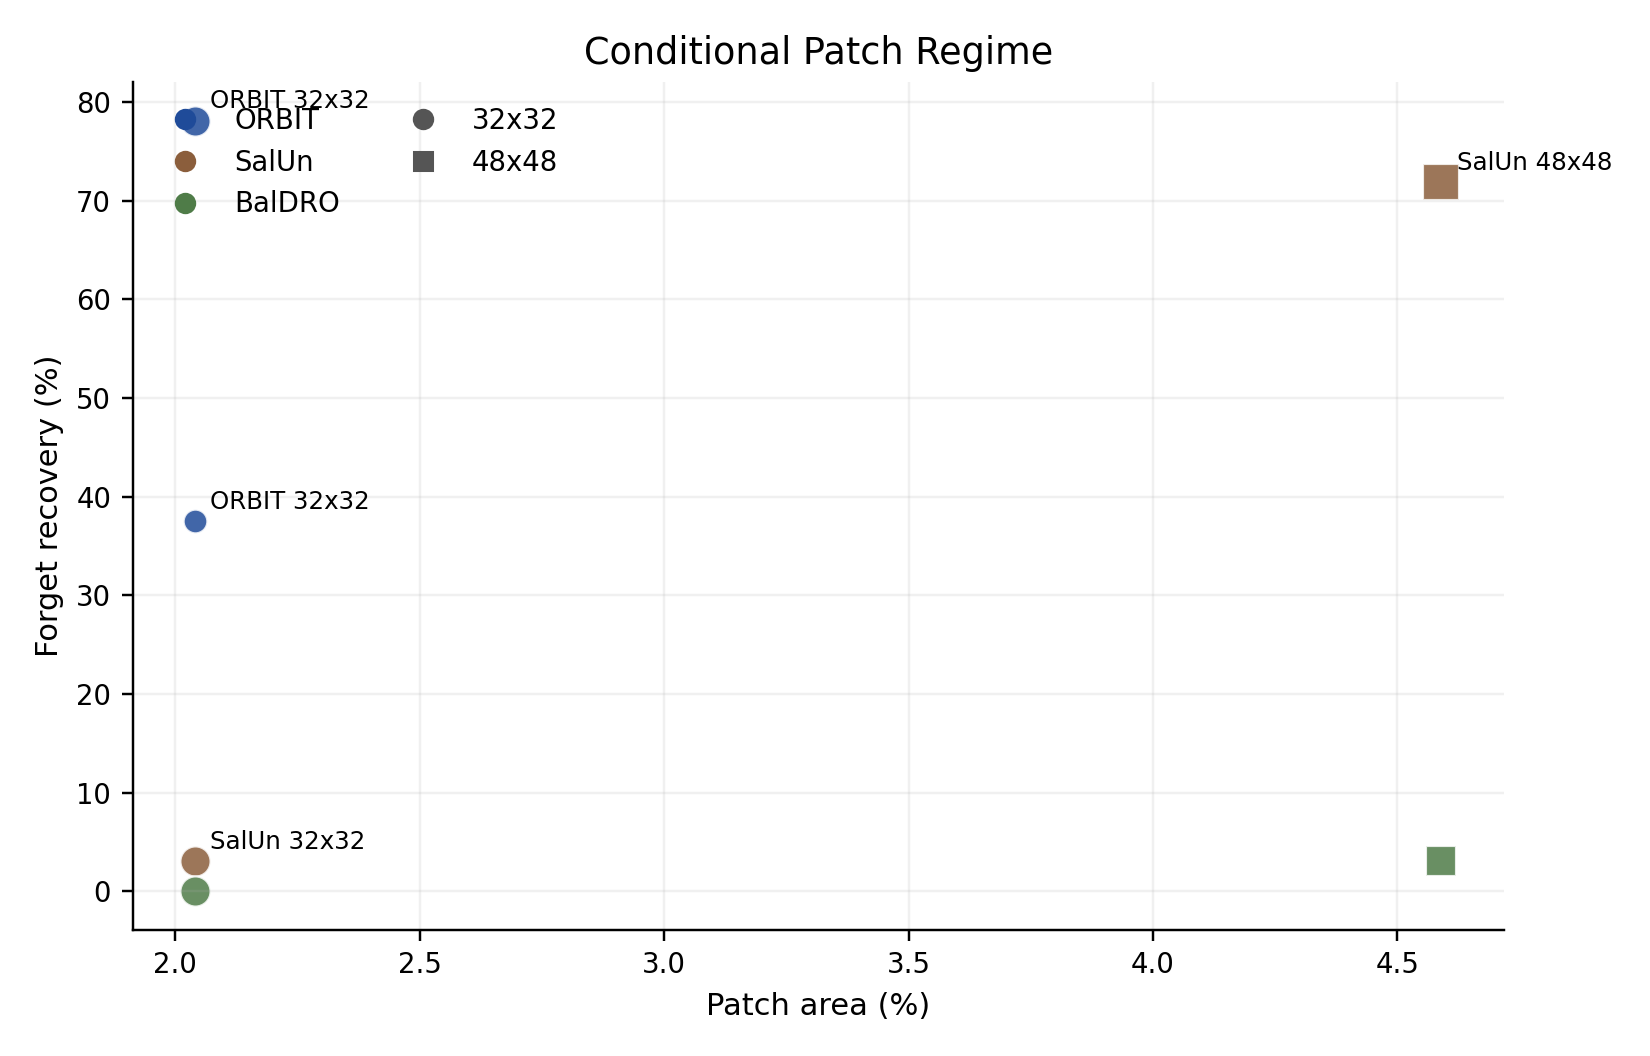
\includegraphics[width=0.9\linewidth]{conditional_patch_regime.png}
  \caption{Conditional patch regime. Point size reflects retain accuracy drop.}
  \label{fig:patch-regime}
\end{figure}
